%% 这是主文件,请以此文件为主开始编排论文格式。
%% 此模板由重庆邮电大学教务处监制。
%% 编者:教务处,李茜,等;计算机学院,卢星宇,刘媛媛,等。
%% 特别感谢2022届先进制造工程学院,张治勇对初版Latex模板的大量贡献。
%% 若有任何格式错误问题或者对Latex模板的改进建议,请联系编者,欢迎各位老师同学一起完善重邮Latex模板。
%% 编译指令: xelatex
\documentclass[UTF8,twoside,zihao=-4,AutoFakeBold,scheme=chinese,openany]{ctexbook}
\usepackage{graphicx}
\usepackage[final]{pdfpages}
% 设置页边距
\usepackage{geometry}
\usepackage{makecell}
\usepackage{caption}
\usepackage{multirow}
\usepackage{booktabs}
\makeatletter
\let\c@lofdepth\relax
\let\c@lotdepth\relax
\makeatother
\usepackage{subfigure}
\usepackage{float}
\usepackage[titles,subfigure]{tocloft}
\usepackage{soul}
\usepackage{color,xcolor}

\usepackage{fontspec}
\setmainfont{Times New Roman}


\geometry{a4paper,top=3cm,bottom=2.5cm,left=2.5cm,right=2.5cm}

% 设置行间距 1.5倍
\linespread{1.5}\selectfont
% 设置段与段之间的垂直距离 \parskip默认橡皮长度是0pt plus 1pt
\setlength{\parskip}{0pt}
% \setlength{\parindent}{0pt}

%设置字体
% 设置英文字体
%\setmainfont{Times New Roman}[
   % BoldFont = Times New Roman Bold,
   % ItalicFont = Times New Roman Italic,
    %BoldItalicFont = Times New Roman Bold Italic
%]

%\setsansfont{Times New Roman}[
    %BoldFont = Times New Roman Bold,
   % ItalicFont = Times New Roman Italic,
    %BoldItalicFont = Times New Roman Bold Italic
%]

%\setmonofont{Times New Roman}[
   % BoldFont = Times New Roman Bold,
   % ItalicFont = Times New Roman Italic,
   % BoldItalicFont = Times New Roman Bold Italic
%]

%设置字号
\usepackage{ctexsize,type1cm}
\newcommand{\yihao}{\fontsize{26pt}{39pt}\selectfont}
\newcommand{\xiaoyi}{\fontsize{24pt}{36pt}\selectfont}   
\newcommand{\erhao}{\fontsize{22pt}{33pt}\selectfont}          
\newcommand{\xiaoer}{\fontsize{18pt}{27pt}\selectfont}          
\newcommand{\sanhao}{\fontsize{16pt}{24pt}\selectfont}        
\newcommand{\xiaosan}{\fontsize{15pt}{22.5pt}\selectfont}        
\newcommand{\sihao}{\fontsize{14pt}{21pt}\selectfont}            
\newcommand{\xiaosi}{\fontsize{12pt}{18pt}\selectfont}            
\newcommand{\wuhao}{\fontsize{10.5pt}{15.75pt}\selectfont}
\newcommand{\xiaowu}{\fontsize{9pt}{13.5pt}\selectfont}    
\newcommand{\liuhao}{\fontsize{7.5pt}{11.25pt}\selectfont}

%使用公式,表格,图片
\usepackage{mathtools,amsmath,amssymb,graphicx,array,float}

% 设置页眉面脚
%% 设置章节前的页码格式
%\usepackage[pagestyles]{titlesec}
%\newpagestyle{MyStyle}{
%  \setfoot{}{\Roman{page}}{}
%%  \headrule
%}

\usepackage{fancyhdr}

\fancypagestyle{content}{
	\fancyhf{}
	\renewcommand{\headrulewidth}{0pt}
%	\renewcommand{\footrulewidth}{0mm}
	\fancyfoot[C]{\songti\xiaowu  \Roman{page}}
}

%重新设置摘要的页码
%\fancypagestyle{content}{
%	\fancyhf{}
%	%   \fancyfoot[C]{\songti\xiaowu  \thepage }
%	%\fancyhead[L]{\songti\xiaowu 硕士学位论文}
%	%    \fancyhead[CE]{\songti\xiaowu 目录 }
%	\fancyfoot[C]{\songti\xiaowu  \Roman{page} }
%}


%重新设置headings
\fancypagestyle{headings}{
    \fancyhf{}
%   \fancyfoot[C]{\songti\xiaowu  \thepage }
   %\fancyhead[L]{\songti\xiaowu 硕士学位论文}
%    \fancyhead[CE]{\songti\xiaowu 目录 }
	\fancyfoot[C]{\songti\xiaowu  \Roman{page} }
	\renewcommand{\headrulewidth}{0.5pt}
	\fancyhead[CO]{\songti\xiaowu 目录 }
	\fancyhead[CE]{\songti\xiaowu 重庆邮电大学本科毕业设计(论文)}
}

%重新设置plain
%正文页眉设置
\fancypagestyle{plain}{
    \fancyhf{}
    \fancyfoot[C]{\songti\xiaowu  \thepage }
    \fancyhead[CO]{\songti\xiaowu \leftmark }
    \fancyhead[CE]{\songti\xiaowu 重庆邮电大学本科毕业设计(论文)}
}

%设置双线页眉
%\makeatletter
%\def\headrule{
%    {\if@fancyplain\let\headrulewidth\plainheadrulewidth\fi%
%    \hrule\@height 1.0pt \@width\headwidth\vskip1pt%上面线为1pt粗
%    \hrule\@height 0pt \@width\headwidth  %下面0.5pt粗
%    \vskip-2\headrulewidth\vskip-1.2pt}    %两条线的距离1pt
%    \vspace{6mm}}     %双线与下面正文之间的垂直间距
%\makeatother

%设置双线页脚
\makeatletter
\def\footrule{
    {\if@fancyplain\let\footrulewidth\plainfootrulewidth\fi%
    \hrule\@height 0pt \@width\headwidth          %上面0.5pt粗
    \vskip 1pt
    \hrule\@height 0pt \@width\headwidth %下面线为1pt粗
    \vskip-2\headrulewidth\vskip-1.2pt}    %两条线的距离1pt
    \vspace{8mm}}     %双线与下面正文之间的垂直间距
\makeatother

%设置文章格式
\ctexset {
    contentsname={目录},
    listfigurename={插图},
    listtablename={表格},
    figurename={图},
    tablename={表},
    bibname={参考文献},
    appendixname={附录},
    chapter={
        beforeskip={0pt},
        nameformat={\heiti\sanhao\centering},
        titleformat={\heiti\sanhao\centering},
    },
    section={
        format={\heiti\sihao},
    },
    subsection={
        format={\heiti\xiaosi},
    },
    subsubsection={
        format={\heiti\xiaosi},
    }
}

% 目录中的章加点
\usepackage[titles]{tocloft}
\renewcommand{\cftdot}{$\cdot$}
\renewcommand{\cftdotsep}{1.5}
\setlength{\cftbeforechapskip}{10pt}

\renewcommand{\cftchapleader}{\cftdotfill{\cftchapdotsep}}
\renewcommand{\cftchapdotsep}{\cftdotsep}
\makeatletter
\renewcommand{\numberline}[1]{%
\settowidth\@tempdimb{#1\hspace{0.5em}}%
\ifdim\@tempdima<\@tempdimb%
  \@tempdima=\@tempdimb%
\fi%
\hb@xt@\@tempdima{\@cftbsnum #1\@cftasnum\hfil}\@cftasnumb}
\makeatother

% 设置目录字体尺寸
\renewcommand{\cftchapfont}{\heiti\xiaosi}
\renewcommand{\cftsecfont}{\heiti\wuhao}
\renewcommand{\cftsubsecfont}{\heiti\wuhao}

%使用代码排版包
\usepackage{listings}
\usepackage{color}
\lstset{%
    frame=shadowbox,
    extendedchars=false,            % 不使用xelatex而使用CJK方式处理汉字
    language=python,
    basicstyle=\sffamily,           % 设置整体格式
    keywordstyle=\bfseries,         % 关键字格式
    commentstyle=\rmfamily\itshape, % 注释格式
    stringstyle=\ttfamily,          % 字符串格式
    columns=flexible,
    escapechar=',                   % 注释中显示汉字,eg //'一个整数'
    tabsize=4,
    numbers=left,
    numberstyle=\small,             % 行号字体设置
    stepnumber=1,                   % 行号距离设置,1代表每行加行号
    numbersep=8pt,                  % 行号和代码距离设置
    backgroundcolor=\color{white},
    showspaces=false,               % show spaces adding particular underscores
    showstringspaces=false,         % 使用下划线连接字符串
    showtabs=false,
    frame=single,                   % 给代码加边框
    captionpos=b,                   % sets the caption-position to bottom
    breaklines=true,                % 自动换行设置
    breakatwhitespace=false,        % sets if automatic breaks should only happen at whitespace
    escapeinside={\%*}{*)},         % if you want to add a comment within your code
    xleftmargin=2em,                % 设置左边距,宽度默认是与页芯等宽的
    xrightmargin=2em,               % 设置右边距,宽度默认是与页芯等宽的
    aboveskip=1em                   % 设置上边距
}

%设置自定义变量
\newcommand\degree{^\cire}

% 定义文献引用格式,\cite正常引用 \supercite右上角引用
\usepackage{cite}
\newcommand{\upcite}[1]{\textsuperscript{\textsuperscript{\cite{#1}}}}
\newcommand\supercite[2][]{%
\textsuperscript{\cite[#1]{#2}}
}

\usepackage{enumitem}
\setlist[description]{
    itemsep=-5pt,
    font=\songti,
}

% 定义中文封面环境
\newenvironment{titletabbing}
{\par\bfseries\songti\sihao\tabbing}
{\endtabbing\par}

\usepackage[nottoc]{tocbibind}
\endinput


\begin{document}
\pagestyle{empty}
% 中文封面页
% !TEX root = main.tex

% 中文封面页, 不能单独编译
% 格式要求:无页眉页脚, 单独成页,后面空一页
\begin{center}
        \newcommand{\settingone}[1]{{\songti\sihao\bfseries #1}}
        \noindent {\songti\sanhao\bfseries    } \hfill
        \newlength{\Mylen}
        \settowidth{\Mylen}{\settingone{学\qquad 号:2022220054}}
        \begin{minipage}[t]{\Mylen} \sihao
                \bfseries 编\qquad 号 : \underline{\phantom{XXXXXX}} \\ 
                \bfseries 审定成绩 : \underline{\phantom{XXXXXX}}
        \end{minipage}
         \\ [1mm]
        \newlength{\Mylentwo} 
        \begin{figure*}[h]
        	\centering
        	
\includegraphics[scale=0.8]{chapters/logo1.jpg}
        \end{figure*}
        %{\yihao\bfseries 重庆邮电大学} \\[3mm]
        {\yihao\bfseries 本科毕业设计(论文)}\\[1mm]
        \begin{figure*}[h]
        	\centering
        	
\includegraphics[scale=0.2]{chapters/logo2.jpg}
        \end{figure*}

		\begin{table}[h]
		\centering
		\renewcommand\arraystretch{1.25}
		\begin{tabular}{p{2cm}p{9cm}}
			\makecell[c]{\bfseries\sihao 中文题目}	& \makecell[c]{\bfseries\sihao 基于Django的宠物商城设计与实现} \\ 
			\cline{2-2} %表格的水平线绘制命令
			\makecell[c]{\bfseries\sihao 英文题目} 	&  \makecell[c]{\bfseries\sihao Thesis Template}  \\ 
			\cline{2-2}
			&  \makecell[c]{}  \\
			\cline{2-2} 
			\makecell[c]{\bfseries\sihao 学院名称} 	&  \makecell[c]{\bfseries\sihao 现代邮政学院}  \\
			\cline{2-2} 
			\makecell[c]{\bfseries\sihao 学生姓名} 	&  \makecell[c]{\bfseries\sihao 罗忠烨}  \\
			\cline{2-2} 
			\makecell[c]{\bfseries\sihao 专\qquad 业} 	&  \makecell[c]{\bfseries\sihao 电子商务}  \\
			\cline{2-2} 
			\makecell[c]{\bfseries\sihao 班\qquad 级} 	& \makecell[c]{\bfseries\sihao  Z0322202} \\
			\cline{2-2} 
			\makecell[c]{\bfseries\sihao 学\qquad 号} 	&  \makecell[c]{\bfseries\sihao 2022220054}  \\
			\cline{2-2} 
			\makecell[c]{\bfseries\sihao 指导教师} 	&  \makecell[c]{\bfseries\sihao 卢华玲  职称}  \\ 
			\cline{2-2}
			\makecell[c]{\bfseries\sihao 答\hspace{6pt}辩\hspace{6pt}组} \\[-2mm] \makecell[c]{\bfseries\sihao 负\hspace{6pt}责\hspace{6pt}人} 	&  \makecell[c]{\bfseries\sihao 姓名  职称}  \\
			\cline{2-2}
		\end{tabular}
	\end{table}
	\vspace{0.1cm}
			\bfseries\sihao 2024 年\hspace{12pt}月
						\\[2mm]
						\bfseries\sihao 重庆邮电大学教务处制
\end{center}


%	\includepdf{moban.pdf} 


% 原创性声明
%% 原创性声明

%\newpage
%\begin{center}\heiti\sanhao
%
%    上海工程技术大学\\
%    学位论文原创性声明
%\end{center}

%\vspace{3em}
%
%本人郑重声明:所递交的学位论文,是本人在导师的指导下,独立进行研究工作
%所取得的成果。除文中已经注明引用的内容外,本论文不包含任何其他个人或集体已
%经发表或撰写过的作品成果。对本文的研究做出重要贡献的个人和集体,均已在文中
%以明确方式标明。本人完全意识到本声明的法律结果由本人承担。

%\vspace{5cm}
%\hspace{10cm}学位论文作者签名:

%\hspace{10cm}日期:\qquad 年 \qquad 月 \qquad 日 
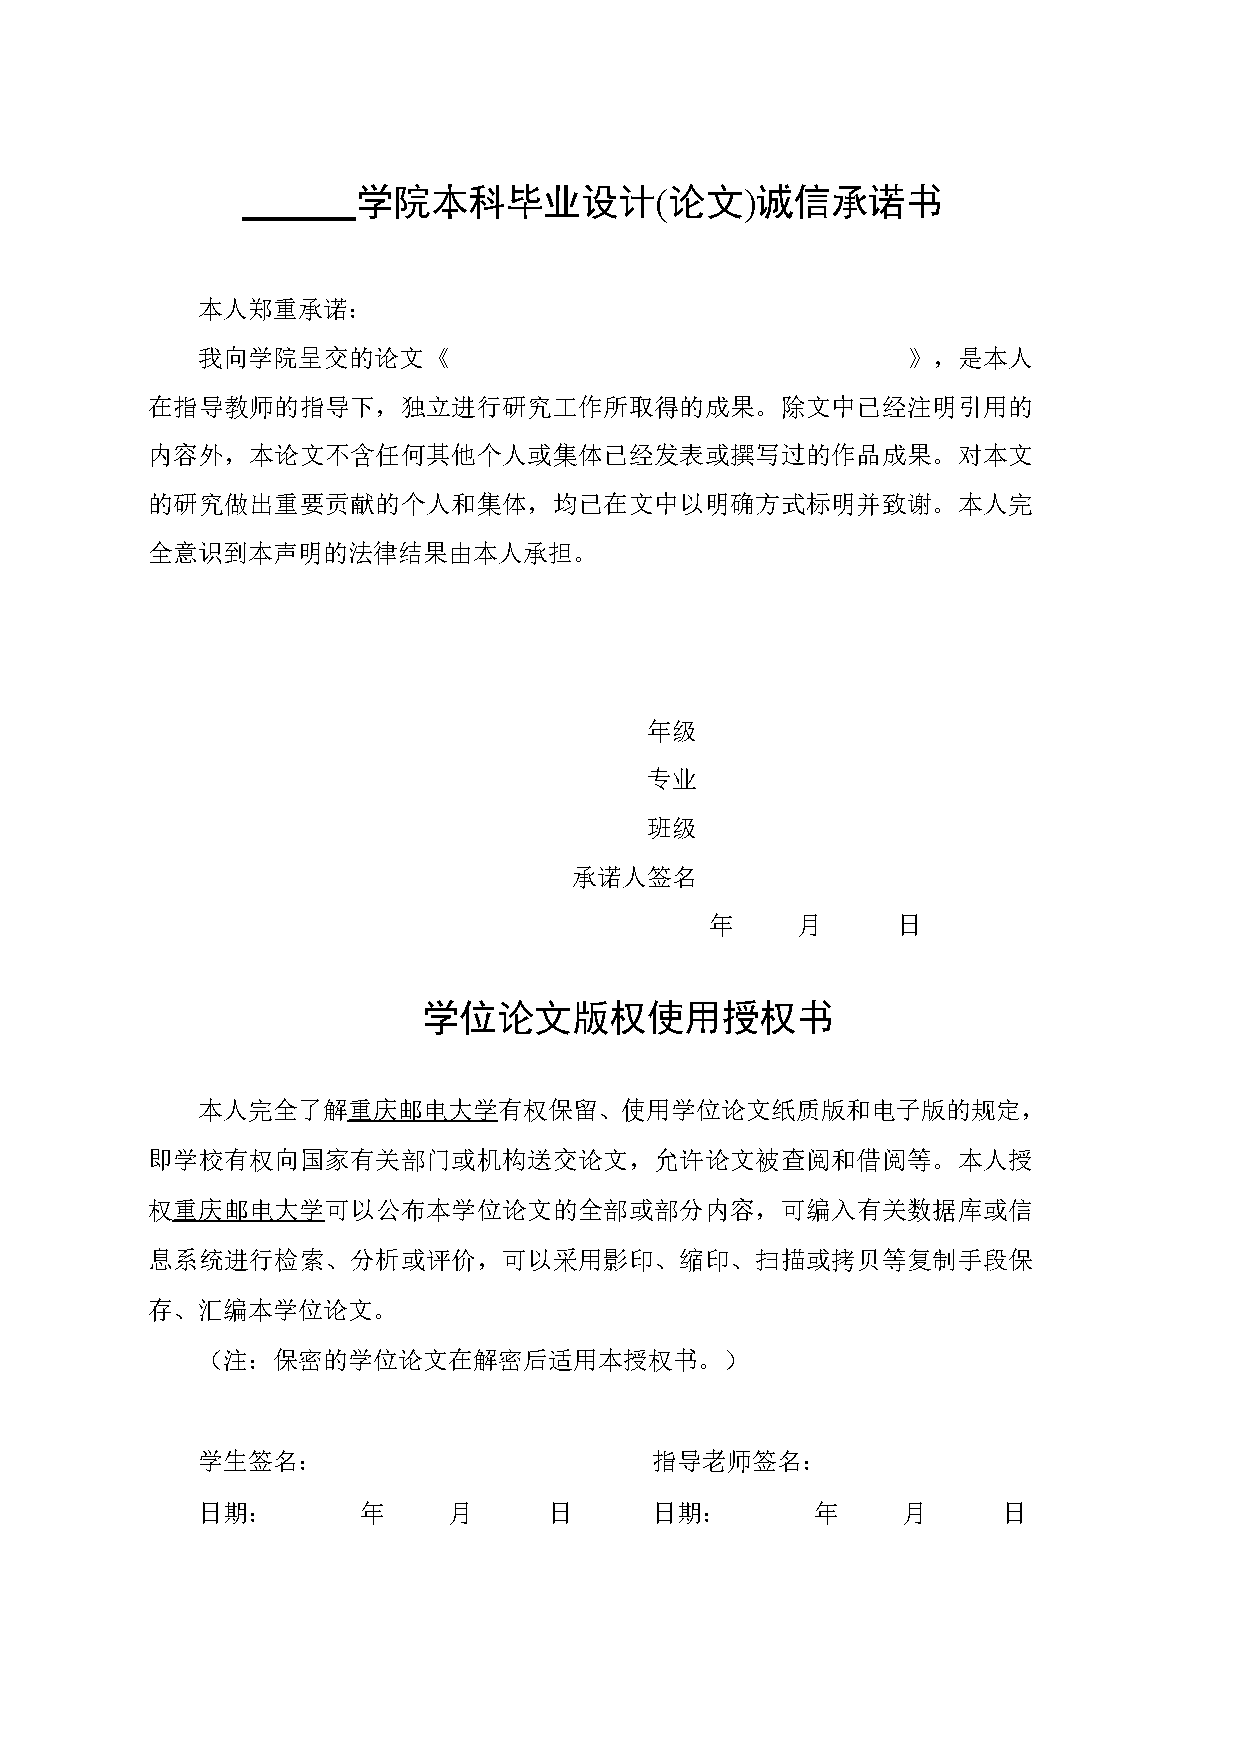
\includepdf{moban2.pdf}


\frontmatter
\pagestyle{content}
%% 中文摘要页


\begin{center}\heiti\sanhao\textbf{
        摘要
    }
\end{center}

毕业设计是本科教学过程最后阶段的一种总结性实践教学环节。通过毕业设计,学生可以综合应用所学的各种理论知识和技能,进行全面、系统、严格的技术及基本能力的练习。为了提高毕业设计论文的质量,做到论文在内容和格式上的规范化与统一化,特制作本模板。
论文摘要是论文内容不加注释和评论的简短陈述,应以第三人称陈述,用语力求简洁、准确。中文摘要字数原则上为400-600字,英文摘要应与中文内容一致。

摘要是学位论文的浓缩,应具有独立性和自含性,即是一篇完整的短文,不阅读论文的全文,就能获得必要的信息。摘要内容应尽可能包括原论文的主要信息,包括研究工作的目的意义、主要问题、研究内容、研究方法、研究结果、主要结论,供读者确定有无必要阅读全文,也供文摘汇编等二次文献采用。摘要要用文字表达,不用图、表、化学结构式、公式、非公知公用的符号和术语。 

关键词是为了文献标引工作从论文中选取出来用以表示全文主题内容信息的单词或术语。自定义3-5个关键词,按外延由大到小排列,建议采用EI标准检索词,关键词间用逗号分开。如有可能,应尽量用《汉语主题词表》等词表提供的规范词。

“摘要”二字为黑体三号字居中,是一级标题。摘要与内容之间不空行,摘要内容与关键词间空一行。“关键词”三个字采用宋体小四号字加粗。摘要内容和关键词采用中文宋体、英文Times New Roman,小四号字,1.5倍行距。\\



  
\quad \noindent \textbf{关键词:}毕业设计,论文格式,规范化,模板

\clearpage
%% 英文摘要页
%% 英文摘要页



\begin{center}\heiti\sanhao\textbf{
        Abstract
    }
\end{center}

Abstract is a brief statement of the thesis without notes and comments, which should be stated in the third person with concise and accurate language in 600-800 Chinese characters and less than 700 words in foreign languages. The writing of an abstract should follow these principles:

1. Abstract should generally state out clearly the purpose, significance, problem, methods, results, main conclusion and its significance, creative achievements and new insights of the research program, and the results and conclusions should be emphasized. 

2. Abstract should be independent and self contained, which can offer the necessary information without reading the full text. It is the miniature and abbreviation of a thesis, which contains the thesis’s main points, views and conclusions in a short and clear way. Abstract is a complete short essay with data and conclusion, which can be adopted and referred to independently. 

3. Abstract should include main information of the original thesis as far as possible for the reader to determine whether to read the full text, which can also be applied for secondary sources. 
4. Abstract should be written in words without any appended drawings and photos. Unless there is no alternative way available, abstract should be presented without graphs, tables, chemical structural equations, non-public common symbols and terminology, subscripts, and other special symbols. It is the best policy to highlight the key points clearly with less data tables.

Keywords are words or terms selected from the thesis for literature indexing to represent the topic information entry. Generally, a thesis should have 3-5 keywords, which should be arranged from broad to narrow entry according to the principle of epitaxial order. EI standard retrieval words are recommended. The keywords should be separated by a comma and there is no punctuation after the last word. If possible, it is better to use the standard words from Chinese Thesauri and other dictionaries of the same type. 

Abstract should be centered in bold-3 word size. It is the primary heading without any blank line between the word “abstract” and its content. But there should be one blank line between the abstract content and the key words. The “keywords” should be in bold Song typeface with small-four word size. The content and the key words are written in Chinese song typeface, English Times New Roman, small-four word size and 1.5 spaced.\\

\quad \noindent \textbf{KEY WORDS:} thesis, format, standardization, template

\clearpage
%% 目录
\pagestyle{headings}
\tableofcontents
%\thispagestyle{MyStyle}
\clearpage
%%===============================
%% 开始章节写作,显示特定页眉页脚
\mainmatter
\pagestyle{plain}
%% 第1章
%% chapter-1: 绪论部分
%% 介绍本研究课题的学术背景及理论与实际意义,国内外文献综述,
%% 本研究课题的来源及主要研究内容。

\chapter{引言}

\section{研究背景和意义}
随着我国宠物养育数量的不断增加和宠物市场的多元化发展,宠物行业正在经历着快速增长的阶段。根据亚宠研究院发布的《宠物行业蓝皮书-2023宠物行业发展报告》,2018-2022年我国的养宠数量持续上升,养宠市场规模不断扩大,成为一个高速发展的行业。该报告预测,到2023年,我国养宠数量将达到近2.0亿只,市场规模将突破2500亿元。

宠物市场的发展呈现出多元化的趋势,消费者洞察显示,养宠人群主要以90后为主,他们更倾向于通过线上渠道购买宠物用品和服务。这一趋势的崛起在一定程度上推动了宠物行业电商化的发展,为市场注入了活力。然而,一些宠物商店仍然只专注于线下零售渠道,可能由于技术水平的不足、资金有限或者观望市场趋势而错失了在线市场的机会,因为越来越多的消费者选择在网上购物。

“十三五”时期,我国电子商务取得了显著成就:电子商务交易额从2015年的21.8万亿元增至2020年的37.2万亿元;全国网上零售额2020年达到11.8万亿元,我国已连续8年成为全球规模最大的网络零售市场;2020年实物商品网上零售额占社会消费品零售总额的比重接近四分之一,电子商务已经成为居民消费的主渠道之一;电子商务从业人员规模超过6000万,电商新业态、新模式创造了大量新职业、新岗位,成为重要的“社会稳定器”。这些数据充分说明,电子商务已经全面融入我国生产生活各领域,成为提升人民生活品质和推动经济社会发展的重要力量。与此同时,我国电子商务发展仍然面临不规范、不充分、不平衡的问题,平台企业垄断和不公平竞争问题凸显,企业核心竞争力不强,外部宏观环境发生复杂深刻变化,电子商务高质量发展机遇和挑战并
存。

党中央、国务院高度关注电子商务的发展,在《“十四五”电子商务发展规划》中明确指出电子商务是大有可为的,并在各个层面提出了促进电子商务发展的要求。特别是在抗击新冠肺炎疫情过程中,电子商务发挥了重要作用,加速了线上线下融合的趋势,
为经济发展注入了新的活力。

在“十四五”规划提出了总体要求,指导思想强调以新发展理念为核心,坚持守正创新、规范发展,推动电子商务与各产业深度融合,通过数字化手段赋能经济社会转型,保障安全健康发展,实现普惠共享与开放共赢的目标。

在当前宠物市场多元化以及电商行业大有可为的背景下,设计和实现一个宠物在线商城是一个具有潜力的创新举措。通过搭建宠物商城平台,不仅可以更好地满足广泛养宠人群的需求,提供全方位的宠物商品和服务,还有助于增加商家的盈收并提高管理效
率。这样的举措不仅能够顺应市场趋势,也为宠物行业的未来发展打开了新的可能性。

本课题旨在通过基于Django的宠物商城设计与实现,满足宠物主人对购物的便捷需求,提高宠物商家的经营效益。具体目的和意义如下:

(1)提升用户体验:通过设计直观、易用的UI界面,提供便捷的商品浏览、购买、支付等功能,提升用户在宠物商城的购物体验。

(2)优化商家管理:提供商家端的管理系统,包括商品管理、订单管理、库存管理等功能,协助商家更高效地运营宠物商城。

(3)提升市场竞争力:在宠物用品市场日益竞争激烈的情况下,通过提供简便易用的宠物商城平台,帮助小型宠物商家在市场中更好地立足和竞争。

(4)促进本地宠物社群互动:通过商城中的评论、社交分享等功能,促进宠物主人之间的互动,形成本地宠物社群,增进用户黏性。


\section{国内外研究现状}
\subsection{国外研究现状}
\textbf{1)分类号}

分类号指中图分类号,是指采用《中国图书馆分类法》(原称《中国图书馆图书分类法》,简称《中图法》)对科技文献进行主题分析,并依照文献内容的学科属性和特征,分门别类地组织文献,所获取的分类代号。采用1999年出版的第四版《中图法》可以在http://www.33tt.com/tools/ztf(中国图书馆分类法中图分类号查询系统)或http://lib.jzit.edu.cn/sjk/tsflf/index.htm(中图法第四版计算机辅助分类查询系统)中查询。填写要求:要求分类细分到22个大类代码后三位数字。如:TN929。

\textbf{2) UDC编号	}

UDC即国际十进分类法(Universal Decimal Classification),是国际通用的多文种综合性文献分类法。UDC采用单纯阿拉伯数字作为标记符号。它用个位数(0~9)标记一级类,十位数(00~99)标记二级类,百位数(000~999)标记三级类,以下每扩展(细分)一级,就加一位数。每三位数字后加一小数点。如电气工程类的论文,其UDC编号为:621.3。


\subsection{国内研究现状}
论文中文题名是以最恰当、最简明的词语,反映学位论文最重要的特定内容的逻辑组合。题名用词应有助于选关键词和编制题录、索引等二次文献,可以提供检索的特定实用信息。题名应恰当简洁,一般不超过25个字。题名应避免使用不常见的缩写词、首字缩写字、字符、代号及公式等。题名语意未尽时,可以用副标题补充说明论文中的特定内容[1]。题名中文宋体,英文Times New Roman小二号字。


\section{研究主要内容}
写出论文的主要工作内容,并逐一介绍每章的内容安排。全文共分为5章,内容结构安排如下:

第1章为引言,引入课题的研究背景及意义….

第2章是天线基本理论分析,….

第3章是设计仿真,….

第4章为优化与分析,….

第5章作为论文的结束语,总结毕业设计工作,提出可以在今后继续深入研究的方向。
\section{研究方法}
文献研究法等
\section{技术路线图}


%% 第2章
%% chapter-2:系统开发关键技术


\chapter{系统开发关键技术}

\section{开发语言:Python}
作为宠物商城系统的主要开发语言,Python凭借其丰富的语言特性使其非常适合快速构建复杂的业务系统。

Python是一门动态类型语言,这意味着变量不需要像Java那样提前声明数据类型,能够在运行时根据赋值自动推断类型。这大大提高了开发的效率,使得程序员可以更专注于业务逻辑,而无需过多考虑类型声明和转换的问题。动态类型也使Python代码更加简洁和灵活,非常适合在原型开发和需求变更频繁的场景中使用。

Python也是一门解释型语言,程序可以逐行执行而无需事先编译。这种交互式的执行模式非常适合进行实验性编程和快速调试。在宠物商城系统开发过程中,笔者广泛地利用了Python的解释性,从而能够快速验证假设,测试新的功能点,缩短反馈循环。

此外,Python拥有出色的跨平台能力。无论是Windows、macOS还是Linux,Python程序几乎可以在任何操作系统上运行而且无需修改代码。这大大提高了系统部署的灵活性,工程师可以在各种环境下进行开发和测试,确保最终产品能够稳定运行在生产环境。

Python的面向对象特性也极大地支持了系统设计。通过类和继承机制,复杂业务可以被划分为清晰的对象模型,并基于这些模型实现面向对象的程序设计。比如在实现支付、物流等功能时,可以定义payment、logistics等抽象类,方便后续拓展不同的具体实现。Python的多态特性则使得这些对象可以透明地互相协作,增强了系统的灵活性。

最重要的是,Python拥有丰富的标准库和第三方库,无需开发者重复造轮子。内置标准库提供了从文件IO、网络编程到数据分析等各种功能,几乎涵盖了系统开发的方方面面。第三方库更是为Python注入了无穷活力,如Django用于Web开发、NumPy用于科学计算、Pyecharts用于数据可视化等。笔者充分地利用了这些优秀的Python库,缩短了开发周期,提高了系统的可靠性。

总而言之,Python拥有卓越的语言特性,包括动态类型、解释执行、跨平台支持、面向对象编程以及丰富的生态圈,都令其成为宠物商城系统开发的最佳选择。这些特性不仅提高了开发效率,也确保了系统具有良好的扩展性和维护性。

\section{后端框架:Django}
Django是本系统使用的后端Web框架,它采用了经典的Model-Template-View (MTV)架构模式。这一模式将系统的职责清晰地划分为3个核心层次。

Model层负责与数据库交互,定义数据模型并实现对数据的增删改查。Django的Object-Relational Mapping (ORM)工具能够将Python对象映射到数据表,极大地简化了数据库操作。在系统设计时,笔者充分利用了Django ORM的特性,如字段类型、关联关系等,设计出符合业务需求的数据模型。

View层实现具体的业务逻辑,接收并处理来自前端的请求,调用Model层完成数据操作,最后返回渲染后的Template。Views可以直接访问Model层的数据,在处理复杂业务时大幅提高开发效率。

Template层负责渲染最终呈现给用户的HTML页面。Templates可以使用Django内置的模板语言,轻松实现动态页面渲染。通过模板继承和组件化,笔者构建了一套高度模块化的前端页面,提升了代码的可维护性。

这三层之间通过明确的接口进行交互,使得系统各个组件高内聚低耦合。比如,Views只需关注业务逻辑,无需关心具体的页面渲染细节;Templates则专注于界面展示,无需处理复杂的后端逻辑。

此外,Django还内置了丰富的功能模块,大大提高了开发效率。例如,自带的用户认证系统能够方便地实现登录注册等功能;表单处理模块简化了与前端的数据交互;管理后台模块则为系统管理员提供了强大的内容管理capabilities。笔者充分地利用了这些Django核心功能,在基础设施建设上节省了大量开发工作。

通过Django强大的模块化设计和丰富的第三方生态,笔者据此引入django-rest-framework实现了基于RESTful API实现数据的传递和交互,同一个API使用不用的请求方式来实现数据的增、删、查、改操作。比如用POST请求实现数据的新增,DELETE请求实现数据的删除,GET请求实现数据的查询,PUT请求实现数据的修改\upcite{Django+Vue.js商城项目实战}。总的来说,Django为宠物商城系统的开发提供了坚实的技术支撑,是系统顺利交付的关键因素之一。

\section{Web前端技术}
宠物商城系统的前端开发采用了HTML、CSS和JavaScript等标准Web技术,并引入了Vue.js前端框架来增强用户体验。

HTML、CSS和JavaScript是构建Web页面的三大基石。HTML定义了页面结构和内容,CSS负责样式渲染,而JavaScript则提供了交互能力。笔者熟练运用这些基础Web技术,搭建了系统的前端界面。例如,使用语义化的HTML标签组织页面布局,通过CSS设计出吸引人的视觉效果,并利用JavaScript实现动态交互,如表单验证、页面路由等。

为了进一步提升前端开发的效率和可维护性,笔者选用了Vue.js作为前端框架。Vue.js提供了声明式渲染、组件系统、路由管理和状态管理等核心功能,大幅改善了前端开发体验。

首先,Vue.js的声明式渲染使得笔者可以以更直观的方式描述页面应该呈现的样子,无需手动操作DOM。这种响应式编程模型能够自动追踪数据变化,并高效地更新相应的界面元素。在宠物商城系统中,笔者广泛应用了Vue.js的数据绑定功能,如商品列表、购物车等均由Vue负责渲染和更新。

其次,Vue.js的组件化思想令前端代码高度模块化。笔者将页面拆分成了各种可复用的组件,如商品详情组件、购物车组件等,极大地提升了代码的可维护性。通过组件的属性传递和事件通信,各个组件之间可以灵活组合,快速构建出复杂的页面布局。

此外,Vue.js内置的路由管理功能帮助笔者轻松实现了多页面的单页应用(SPA)架构。通过定义各种路由规则,笔者可以优雅地处理页面之间的跳转逻辑,而无需自己操作浏览器历史栈。这不仅提升了用户体验,也简化了前端代码。

最后,Vue.js的状态管理机制Vuex进一步增强了笔者的前端开发能力。复杂业务通常需要在多个组件间共享状态,Vuex提供了一个可预测的状态容器,帮助笔者管理这些共享数据。在宠物商城系统中,笔者利用Vuex管理了诸如购物车、用户信息等关键状态,protected数据的一致性和可靠性。

除了Vue.js,笔者还引入了ECharts等数据可视化库,为页面呈现丰富的交互效果和数据分析展示。比如在后台管理模块中,笔者利用ECharts绘制了各种报表和统计图表,帮助管理员更好地洞察业务数据。

\section{关系型数据库:MySQL}
作为宠物商城系统的关系型数据库管理系统,MySQL凭借其出色的性能、可靠性和丰富的生态,非常适合作为系统的数据存储解决方案。

首先,笔者选择MySQL作为数据库,是基于它广泛的应用基础和出色的处理能力。作为开源的关系型数据库,MySQL在Web应用开发领域拥有丰富的使用经验和大量的third-party支持。它能够稳定地支撑起宠物商城系统复杂的数据存储需求,满足高并发访问的性能要求。

其次,笔者充分利用了Django ORM (Object-Relational Mapping)工具,将Python对象seamlessly映射到MySQL数据表。ORM将复杂的SQL操作封装成简单易用的API,大大降低了数据库访问的难度。在系统设计时,笔者根据业务实体定义了一系列Django模型类,通过它们就可以方便地执行增删改查等数据库操作,而无需编写原生的SQL语句。这不仅提高了开发效率,也确保了代码的可移植性,因为无需与特定数据库耦合。

为了满足复杂的业务需求,笔者还充分挖掘了MySQL的高级功能。比如,合理设计数据模型是确保系统数据完整性的关键。笔者仔细分析了各个业务实体之间的关系,采用恰当的数据类型、主键、外键等约束,构建出健壮的数据库schema。同时,笔者还根据业务访问模式,在关键字段上建立索引,大幅提升了数据查询性能。

此外,MySQL强大的存储过程和视图机制也在系统开发中发挥了重要作用。对于一些复杂的数据处理逻辑,笔者将其encapsulate在存储过程中,十分便于重用和维护。而视图则用于提供定制化的数据视角,帮助应用程序更好地满足特定的报表和分析需求。

MySQL作为宠物商城系统的关系型数据库,为笔者提供了稳定可靠的数据存储能力。通过Django ORM的抽象,笔者简化了与数据库的交互;同时充分利用MySQL的高级特性,进一步优化了系统的数据处理能力。可靠的数据存储是支撑整个宠物商城系统运转的基础,因此MySQL的优秀表现功不可没。

\section{集成开发环境:PyCharm}
作为宠物商城系统的主要集成开发环境(IDE),PyCharm提供了丰富的功能,极大地提升了笔者在整个开发过程的效率和质量。

PyCharm的代码编辑功能是笔者日常开发的基础。它提供了智能感知、自动补全等便利工具,大幅提高了编码速度。比如,当笔者输入Django模型类的字段名时,PyCharm能够自动列出可用的选项,减少了记忆负担。代码重构功能也为笔者的重构实践提供了强大支持,只需简单的快捷键操作,就能对变量、方法等进行安全可靠的修改。

PyCharm卓越的调试能力帮助笔者快速定位和解决系统bug。它内置了强大的断点调试器,允许笔者在运行时暂停程序、检查变量状态、单步执行等。这在分析复杂的业务逻辑时尤为有用。PyCharm还能自动检测常见的编码错误,及时给出提示,避免了低级错误的产生。

PyCharm对版本控制系统的集成进一步提升了团队协作效率。笔者使用Git作为代码仓库,PyCharm为各种Git操作提供了图形化界面,如查看提交历史、比较文件差异、解决合并冲突等。这些功能大大简化了日常的版本管理工作。

PyCharm还提供了丰富的第三方插件支持,为特定需求扩展了IDE的功能。笔者安装了Django、Pytest等专用插件,它们能够自动识别Django项目结构,提供上下文相关的智能提示和操作。同时,PyCharm也集成了单元测试运行、部署发布等实用工具,使得整个开发生命周期都在IDE中得到支持。

PyCharm作为宠物商城系统的主要开发环境,为笔者带来了显著的效率提升。它强大的代码编辑、调试、版本控制等核心功能,再加上针对Python语言和Django框架的专有特性,极大地方便了日常的开发、测试和部署实践。毋庸置疑,PyCharm是确保该系统顺利交付的重要保障之一。

\section{本章小结}
本章详细介绍了宠物商城系统的关键开发技术,包括Python编程语言、Django后端框架、Vue.js前端框架、MySQL关系型数据库以及PyCharm集成开发环境。这些技术在系统的分析、设计和实现过程中发挥了关键作用。通过采用面向对象的建模方法和全栈开发模式,系统实现了高效灵活的业务逻辑和优秀的用户体验。
%% 第3章
%% chapter-3: 系统分析


\chapter{系统分析}
\section{系统需求分析}
\subsection{系统功能性需求分析}

\subsection{系统非功能性需求分析}


\section{系统可行性分析}


\section{数据流程分析}


\section{本章小结}

 

\chapter{系统设计}

\section{系统总体设计}

学位论文用A4(210×297mm)纸,采用双面打印,装订成品尺寸:207×291mm。

论文外部封面采用学校当年统一印刷提供的封面。此论文模板封面为内封,应是打印论文时的内页首页。评审、答辩等中间环节提供的纸质论文可不用学校统一外封面正式装订,而是用本模板封面作为临时封面。

\section{系统详细设计}

从目录页开始到论文最后一页,均需设置页眉。页眉内容:偶数页居中对齐为“重庆邮电大学本科毕业设计(论文)”,奇数页居中对齐是各章章名;字体采用宋体5号。页眉之下有一条下划线。封面、摘要没有页眉,也没有边框。

\subsection{代码设计}
\subsection{数据库设计}

\section{输入输出设计}
\subsection{系统输入设计}

\subsection{系统输出设计}

\section{本章小结}
介绍了学位论文的其他格式要求,以及学校关于检查论文中非学术性错误(俗称低级错误)的要求。








\chapter{系统实现}


\section{系统部署环境}


\section{系统首页}

\section{前台用户系统}

\section{后台管理系统}

\section{本章小结}













\chapter{系统测试}

\section{系统测试的目的和方法}

参考文献反映论文作者的科学态度和论文具有真实、广泛的科学依据,也反映论文的起点和深度。方便论文作者与前人的成果区别开来,是对他人劳动成果的尊重。方便读者检索和查找有关资料。有利于节省论文篇幅,有助于科技情报人员进行情报研究和计量学研究。

\section{系统功能模块测试}

\section{测试结果及分析}

\section{本章小结}

介绍了参考文献的标注方法、著录方法和相关要求。











\chapter{总结与展望}

学位论文应有结论,可以从论文的主要工作、创新点和后续的研究工作等方面进行总结。

\section{主要工作与创新点}

学位论文的结论是最终的、总体的结论,不是正文中各段的小结的简单重复。结论应该观点明确、严谨、完整、准确、精炼。文字必须简明扼要。可以从论文的主要工作、创新点和后续的研究工作等方面总结。

如果不可能导出应有的结论,也可以没有结论而进行必要的讨论。

可以在结论或讨论中提出建议、研究设想、仪器设备改进意见、尚待解决的问题等。不要简单重复罗列实验结果,要认真阐明本人在科研工作中创造性的成果和新见解,在本领域中的地位和作用,新见解的意义。对存在的问题和不足应作出客观的叙述。应严格区分自己的成果与他人(特别是导师的)科研成果的界限。

一般应按四级标题的方式给出,根据需要设置数量。如本文主要工作和创新点如下:

1)阐述第一个创新工作。不要把阅读文献当成创新工作。

2)阐述第二个创新工作。

3)阐述第三个创新工作。

4)阐述第四个创新工作。

特别提醒,不应简单和中文摘要内容相互拷贝。同一段文字或句子在本文中原则上只出现一次。

\section{后续研究工作展望}

针对工作不足或问题,说明更下一步深入的研究。如内容较多,也应用四级标题方式列出。
\backmatter
%% 参考文献
%% 参考文献使用
%设置参考文献风格,参照使用 https://github.com/Haixing-Hu/GBT7714-2005-BibTeX-Style

% 参考文献呈现方式
\bibliographystyle{unsrt}

% .bib文件名  此参考文献在文件夹chapters下,名为ref.bib文件

\bibliography{ref}
%% 致谢
%% 致谢

\chapter{致谢}

{\songti\xiaosi
致谢二字一级标题:黑体3号字居中,段前17磅,段后16.5磅,1.5倍行距,致谢二字与致谢内容之间不空行。致谢内容正文样式:宋体小四号,1.5倍行距。
可以从下列方面致谢:协助完成研究工作和提供便利条件的组织或个人;在研究工作中提出建议和提供帮助的人;给予转载和引用权的资料、图片、文献、研究思想和设想的所有者;其他应感谢的组织或个人。
主要感谢导师和对论文工作有直接贡献及帮助的人士和单位。学位申请人的家属及亲朋好友等与论文无直接关系的人员,一般不列入致谢的范围。
致谢辞应谦虚诚恳,实事求是,切忌浮夸与庸俗之词。 }


%\vspace{8cm}
%\begin{flushright}
%    年 \qquad 月

    %于重庆邮电大学
%\end{flushright}
%}
%% 附录
%% 附录页

\chapter{附录A\quad 科技写作中非学术型低级错误的主要表现}
% \addcontentsline{toc}{chapter}{附录}

%{%
%\noindent\songti\xiaosi\textbf{1.\ xxx} 
%
%\noindent xxxxxxxxxxxxx
%
%\noindent \textbf{2.\ xxx}
%\noindent xxxxxxxxxxxxx
%}

本附录主要针对学位论文写作或中文科技论文写作,供重庆邮电大学学位论文查非工作参考。未尽事宜,可参考重庆邮电大学论文写作要求、重庆邮电大学学报编辑部等国内期刊社、出版社的通用出版规定。

推荐阅读《科学出版社作者编辑手册》、《科学道德与学风建设宣传参考大纲(试用本)》等写作指导性书籍或资料,可了解更多、更详尽的通用写作出版规范。
%% 附录页


\chapter{附录B\quad 英文翻译}
% \addcontentsline{toc}{chapter}{附录}

\textcolor{red}{指导教师制定与专业相关的外文文献内容,由学生独立翻译成中文,其外文文献内容翻译成中文后的内容不得少于3000字符。译文和原文附于附录部分,按照正文格式进行排版。若原文没有电子版只是原版的复印件,复印件装订在内可不计页码。}
\end{document}